\documentclass[11pt,a4paper]{article}
\usepackage[margin=2.3cm]{geometry}
\IfFileExists{lmodern.sty}{\usepackage{lmodern}}{}
\usepackage[T1]{fontenc}
\usepackage{titlesec,tabularx,longtable,booktabs,array,enumitem,xcolor,fancyhdr,amsmath}
\usepackage{listings}
\usepackage{tikz}
\usetikzlibrary{arrows.meta,positioning,fit,calc,shapes.geometric,backgrounds}
\usepackage[hyphens]{url}
\usepackage{hyperref}

\definecolor{headcolor}{RGB}{15,70,60}
\definecolor{boxa}{RGB}{226,239,236}
\definecolor{boxb}{RGB}{238,242,250}
\definecolor{boxc}{RGB}{250,243,230}
\definecolor{boxd}{RGB}{245,245,245}
\definecolor{edge}{RGB}{70,70,70}
\hypersetup{colorlinks=true,linkcolor=headcolor,urlcolor=headcolor,
  pdftitle={TrustBazaar System Design - Unit 3: Auction Engine, Listings and Search},
  pdfauthor={S. M. Nihal Ahmed, Afrim Hossen Khan, Sabikun Nahar Sinthia}}

\titleformat{\section}{\normalfont\Large\bfseries\color{headcolor}}{\thesection}{10pt}{}
\titleformat{\subsection}{\normalfont\large\bfseries}{\thesubsection}{8pt}{}
\titleformat{\subsubsection}{\normalfont\normalsize\bfseries}{\thesubsubsection}{6pt}{}
\pagestyle{fancy}\fancyhf{}
\fancyhead[L]{System Design Document}\fancyhead[R]{Unit 3: Auctions, Listings \& Search}
\fancyfoot[C]{\thepage}\renewcommand{\headrulewidth}{0.4pt}\setlength{\headheight}{14pt}
\setlength{\emergencystretch}{3em}
\setlength{\parskip}{0.45em}\setlength{\parindent}{0pt}

\lstdefinelanguage{SQLpg}{morekeywords={CREATE,TABLE,TYPE,AS,ENUM,PRIMARY,KEY,REFERENCES,NOT,NULL,DEFAULT,CHECK,UNIQUE,INDEX,ON,WHERE,TRIGGER,BEFORE,INSERT,UPDATE,DELETE,FOR,EACH,ROW,EXECUTE,FUNCTION,RETURNS,LANGUAGE,BEGIN,END,IF,THEN,ELSE,RETURN,SELECT,FROM,INTO,ORDER,BY,DESC,LIMIT,GRANT,REVOKE,TO,SCHEMA,EXTENSION,EXISTS,OR,AND,IN,IS,ALTER,ADD,FOREIGN,GENERATED,ALWAYS,IDENTITY,DEFERRABLE,INITIALLY,DEFERRED,DECLARE,PERFORM,LOOP,RAISE,EXCEPTION,USING,DISTINCT,ROLE,LOGIN,USAGE,ALL,TABLES,STABLE,DO},sensitive=false,morecomment=[l]{--},morestring=[b]'}
\lstset{basicstyle=\ttfamily\scriptsize,columns=fullflexible,keepspaces=true,breaklines=true,
  keywordstyle=\color{headcolor}\bfseries,commentstyle=\color{gray}\itshape,frame=single,rulecolor=\color{gray!40},
  upquote=true,literate={–}{{--}}1}

\newenvironment{dtable}[1]{\small\begin{longtable}{#1}}{\end{longtable}}

\begin{document}
\begin{titlepage}
\centering
\vspace*{1cm}
{\Large Daffodil International University}\\[0.2cm]
{\large Department of Software Engineering}\\[2cm]
\rule{\linewidth}{0.5pt}\\[0.4cm]
{\huge\bfseries System Design Document}\\[0.3cm]
{\LARGE Unit 3: Auction Engine; Listings, Search \& Fixed-Price}\\[0.3cm]
{\large TrustBazaar: A Verified Peer-to-Peer Auction and Marketplace Platform for Used Goods}\\[0.2cm]
\rule{\linewidth}{0.5pt}\\[1.6cm]
{\large S. M. Nihal Ahmed (232-35-002)\\[0.1cm] Afrim Hossen Khan (232-35-076)\\[0.1cm] Sabikun Nahar Sinthia (232-35-475)}\\[1.6cm]
\begin{tabular}{|l|>{\raggedright\arraybackslash}p{8cm}|}
\hline
\textbf{Status} & Draft for team review \\ \hline
\textbf{Version} & 0.1, 14 October 2026 \\ \hline
\textbf{Implements} & SRS v2.0 (\texttt{docs/srs.tex}) \\ \hline
\textbf{Depends on} & Unit 1 (Identity \& Access), Unit 2 (Order, Payment \& Escrow) \\ \hline
\textbf{Database schema} & \texttt{docs/design/sql/03\_listings\_auctions.sql}, tested on PostgreSQL (67 checks and concurrency tests, Appendix B) \\ \hline
\end{tabular}
\vfill
\end{titlepage}
\tableofcontents
\newpage
\section{Introduction}

\subsection{Purpose}
This document is the third unit of TrustBazaar's System Design Document. It covers two closely linked parts of the SRS:
\begin{itemize}[nosep]
  \item \textbf{listings}: creating and managing listings, photos, categories, screening, search, the featured label, and the stock side of fixed-price purchase;
  \item \textbf{the auction engine}: server-authoritative bidding with proxy maximums, reserve prices and anti-sniping, the live channel to viewers, closing, second-chance offers and non-payment strikes.
\end{itemize}
Acceptance criterion 1 (two simultaneous bids never both win) and the stock half of criterion 2 (no over-sale) depend on this unit.

The unit follows conventions DC-1 to DC-13 (Unit~1 Section~2; Unit~2 Section~2.3) and builds on both earlier units. It uses Unit~1 for identity checks, rate limits, audit and staff actions. It creates auction orders through Unit~2's \texttt{OrdersPort} and provides the stock port that Unit~2's checkout uses.

\subsection{Scope}
\textbf{In scope:}
\begin{itemize}[nosep]
  \item the listing life cycle, photos and the media pipeline, categories and prohibited items, keyword screening, clarifications and listing limits;
  \item visibility of listings when a seller is unverified or suspended;
  \item the stock port: reserve, release and mark sold;
  \item search and filters, distance, sorting and the featured strip;
  \item the auction rules and the bid engine, bid history and bidder masks, the live channel, closing;
  \item second-chance offers, strikes and bidding restrictions, voiding and recomputing bids, and shill-bidding flags.
\end{itemize}

\textbf{Out of scope, owned by later units:}
\begin{itemize}[nosep]
  \item the game-account details and ownership proof (Unit~5, which approves game-account listings through this unit's port);
  \item the delivery of notifications, including outbid notices outside the live channel (Unit~6);
  \item the operator queues and their screens for reviewing listings, reports and flags (Unit~7);
  \item payment of featured fees (Unit~2).
\end{itemize}

\subsection{Requirements covered}
\begin{itemize}[nosep]
  \item \textbf{Functional:} FR-LST-01 to FR-LST-13; FR-SRC-01 to FR-SRC-06; FR-AUC-01 to FR-AUC-18; FR-FIX-02, FR-FIX-04 and FR-FIX-05 (stock side); FR-MON-05 (featured label); FR-KYC-10 and FR-TNS-05 (hiding listings); FR-TNS-02 and FR-TNS-08 (flags).
  \item \textbf{Security:} SEC-ABU-01 (bid and listing limits), SEC-WEB-05 (hidden fields), SEC-DAT-08 and SEC-INP-04 (listing photos), SEC-SES-07 (live channel).
  \item \textbf{Other:} IF-UI-03, IF-COM-02; NFR-PERF-01 to NFR-PERF-03, NFR-PERF-05, NFR-PERF-08; NFR-REL-01, NFR-REL-03; NFR-SCL-01 to NFR-SCL-03; NFR-USE-01; DR-03, DR-04, DR-10.
\end{itemize}

% ------------------------------------------------------------------
\section{Unit Overview}

\subsection{Responsibilities}
\begin{enumerate}[nosep]
  \item Publish only listings that meet the rules: allowed category, photos, defect declaration and parcel details. Lock their content once anyone has bid or bought.
  \item Never sell more units than exist, however many buyers arrive at once.
  \item Find listings quickly in Bangla and English, by text, filters and distance, without revealing exact locations.
  \item Decide every bid under one rule set, in a single serial order per auction, against the server's clock. Publish the result to every viewer within a second.
  \item Close each auction exactly once, create the winner's order, and run second-chance offers and strikes when a winner does not pay.
\end{enumerate}

\subsection{Components}
\begin{figure}[!htbp]
\centering
\resizebox{\textwidth}{!}{%
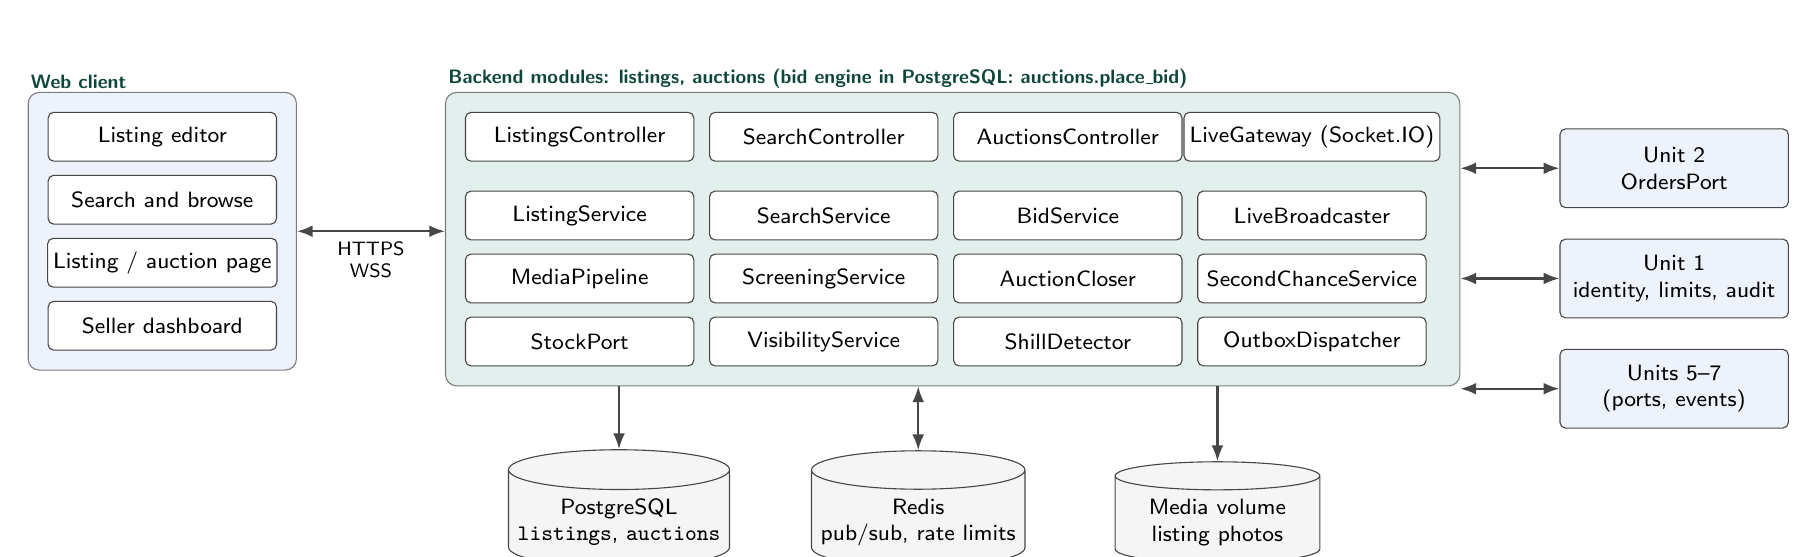
\begin{tikzpicture}[
  font=\sffamily\footnotesize,
  comp/.style={draw=edge, rounded corners=2pt, fill=white, minimum width=2.9cm, minimum height=0.62cm, align=center, inner sep=2pt},
  grp/.style={draw=edge!70, rounded corners=4pt, inner sep=7pt},
  lbl/.style={font=\sffamily\scriptsize\bfseries, text=headcolor, anchor=south west, inner sep=1pt},
  arr/.style={-{Latex[length=2mm]}, draw=edge, thick},
  store/.style={draw=edge, fill=boxd, cylinder, shape border rotate=90, aspect=0.18, minimum width=2.6cm, minimum height=1.1cm, align=center}
]
\node[comp] (c1) at (0,3.9) {Listing editor};
\node[comp] (c2) at (0,3.1) {Search and browse};
\node[comp] (c3) at (0,2.3) {Listing / auction page};
\node[comp] (c4) at (0,1.5) {Seller dashboard};
\begin{scope}[on background layer]\node[grp, fill=boxb, fit=(c1)(c4)] (client) {};\end{scope}
\node[lbl] at (client.north west) {Web client};
\foreach \n/\x/\y/\t in {k1/5.3/3.9/ListingsController, k2/8.4/3.9/SearchController, k3/11.5/3.9/AuctionsController, k4/14.6/3.9/LiveGateway (Socket.IO),
  s1/5.3/2.9/ListingService, s2/8.4/2.9/SearchService, s3/11.5/2.9/BidService, s4/14.6/2.9/LiveBroadcaster,
  s5/5.3/2.1/MediaPipeline, s6/8.4/2.1/ScreeningService, s7/11.5/2.1/AuctionCloser, s8/14.6/2.1/SecondChanceService,
  s9/5.3/1.3/StockPort, s10/8.4/1.3/VisibilityService, s11/11.5/1.3/ShillDetector, s12/14.6/1.3/OutboxDispatcher}
  {\node[comp] (\n) at (\x,\y) {\t};}
\begin{scope}[on background layer]\node[grp, fill=boxa, fit=(k1)(k4)(s9)(s12)] (be) {};\end{scope}
\node[lbl] at (be.north west) {Backend modules: listings, auctions (bid engine in PostgreSQL: auctions.place\_bid)};
\node[store] (pg) at (5.8,-1.0) {PostgreSQL\\\texttt{listings}, \texttt{auctions}};
\node[store] (rd) at (9.6,-1.0) {Redis\\pub/sub, rate limits};
\node[store] (vol) at (13.4,-1.0) {Media volume\\listing photos};
\node[comp, fill=boxb, minimum height=1.0cm] (u2) at (19.2,3.5) {Unit 2\\OrdersPort};
\node[comp, fill=boxb, minimum height=1.0cm] (u1) at (19.2,2.1) {Unit 1\\identity, limits, audit};
\node[comp, fill=boxb, minimum height=1.0cm] (u5) at (19.2,0.7) {Units 5--7\\(ports, events)};
\draw[arr, {Latex[length=2mm]}-{Latex[length=2mm]}] (client.east) -- node[below, font=\sffamily\scriptsize, align=center]{HTTPS\\WSS} (be.west|-client.east);
\draw[arr] (pg.north|-be.south) -- (pg.north);
\draw[arr, {Latex[length=2mm]}-{Latex[length=2mm]}] (rd.north|-be.south) -- (rd.north);
\draw[arr] (vol.north|-be.south) -- (vol.north);
\foreach \t in {u2,u1,u5}{\draw[arr, {Latex[length=2mm]}-{Latex[length=2mm]}] (be.east|-\t) -- (\t.west);}
\end{tikzpicture}}
\caption{Components of the Auctions, Listings \& Search unit. The bid engine's critical section is the database function \texttt{auctions.place\_bid}; Redis carries live messages between backend instances.}
\label{fig:components}
\end{figure}

\begin{dtable}{@{}>{\raggedright\arraybackslash}p{3.4cm}>{\raggedright\arraybackslash}p{11.8cm}@{}}
\toprule
\textbf{Component} & \textbf{Responsibility} \\ \midrule \endhead
ListingService & Create, edit, publish, cancel and clarify listings; enforce the listing limit; record status history. \\
MediaPipeline & Check, strip, resize and store listing photos (Section~\ref{sec:media}). \\
ScreeningService & Match listing text against the screening terms; hold matches for review (FR-LST-11). \\
StockPort & \texttt{reserve}, \texttt{release} and \texttt{markSold} for Unit~2 (DC-13). \\
VisibilityService & Hides and restores a seller's listings on identity events (FR-SRC-04, FR-KYC-10, FR-TNS-05). \\
SearchService & Text search, filters, distance, sorting, featured strip, pagination (Section~\ref{sec:search}). \\
BidService & Checks eligibility and limits, calls \texttt{auctions.place\_bid}, and hands the result to the broadcaster. \\
LiveGateway, LiveBroadcaster & Socket.IO rooms per auction; state messages with sequence numbers; outbid notices. \\
AuctionCloser & Closes due auctions exactly once and creates the winner's order (Section~\ref{sec:close}). \\
SecondChanceService & Strikes, restrictions and second-chance offers after an unpaid win. \\
ShillDetector & Scores bidding patterns and raises flags for operators (FR-AUC-18). \\
\bottomrule
\end{dtable}

\subsection{Why the bid decision runs in the database}
\label{sec:why-db}
The rule ``each bid is evaluated against the state left by the previous one'' (FR-AUC-03) requires the read--decide--write of a bid to be serialised per auction. The decision is therefore a PL/pgSQL function, \texttt{auctions.place\_bid}, which locks the auction row, decides and writes in one database round trip. The service layer keeps everything that does not need the lock: authentication, the KYC gate, rate limits, and the broadcast after commit.

This has three advantages:
\begin{itemize}[nosep]
  \item \textbf{Short lock time.} The lock is held only for the time the function takes, rather than across several network round trips. Measured in the database over 500 accepted bids, a call takes about 0.19~ms, excluding network and commit time.
  \item \textbf{One source of truth.} There is no second lock in Redis that could disagree with the database (NFR-REL-01).
  \item \textbf{Testable rules.} The rules can be tested directly on the database, including under real concurrency (Appendix~\ref{app:tests}).
\end{itemize}
The cost is that this business logic lives in SQL rather than TypeScript. To keep that manageable, the rules are a single pure function, \texttt{auctions.resolve}, used both for live bids and for replay, and the TypeScript tests call the same function.
\section{Interfaces}

\subsection{HTTP API}
\label{sec:api}
All paths are under \texttt{/api/v1}; policies and rate-limit rules are those of Unit~1. Responses never include a bidder's maximum, the reserve amount, a seller's exact coordinates or any bidder's identity (SEC-WEB-05).

{\small
\begin{longtable}{@{}>{\ttfamily\raggedright\arraybackslash}p{1.15cm}>{\ttfamily\raggedright\arraybackslash}p{4.6cm}>{\raggedright\arraybackslash}p{2.7cm}>{\raggedright\arraybackslash}p{6.5cm}@{}}
\toprule
\textnormal{\textbf{Method}} & \textnormal{\textbf{Path}} & \textbf{Policy} & \textbf{Purpose (requirement)} \\ \midrule \endhead
\multicolumn{4}{@{}l}{\textbf{Listings}} \\
GET & /\allowbreak categories & Public & Category tree in Bangla and English; prohibited ones shown as policy only (FR-LST-10) \\
POST & /\allowbreak listings & Verified(list) & Create a draft (FR-LST-01 to 06) \\
PATCH & /\allowbreak listings/\allowbreak \{id\} & Seller & Edit a draft, or an active listing before its first bid or order (FR-LST-07) \\
POST & /\allowbreak listings/\allowbreak \{id\}/\allowbreak photos & Seller & Upload a photo (Section~\ref{sec:media}) \\
DELETE & /\allowbreak listings/\allowbreak \{id\}/\allowbreak photos/\allowbreak \{pid\} & Seller & Remove a photo while editable \\
POST & /\allowbreak listings/\allowbreak \{id\}/\allowbreak publish & Verified(list), seller & Publish, or send for review (FR-LST-11, 12) \\
POST & /\allowbreak listings/\allowbreak \{id\}/\allowbreak clarifications & Seller & Add a time-stamped clarification (FR-LST-07) \\
POST & /\allowbreak listings/\allowbreak \{id\}/\allowbreak cancel & Seller & Cancel where allowed (FR-LST-08) \\
POST & /\allowbreak listings/\allowbreak \{id\}/\allowbreak ai-\allowbreak draft & Seller & Draft text from photos, returned for editing only (FR-LST-13, Could) \\
GET & /\allowbreak listings/\allowbreak \{id\} & Public & Listing page with rounded distance, clarifications, auction state \\
GET & /\allowbreak me/\allowbreak listings & Verified & My listings and their states \\
\multicolumn{4}{@{}l}{\textbf{Search}} \\
GET & /\allowbreak search & Public & Text, filters, sort, cursor (FR-SRC-01 to 05) \\
GET & /\allowbreak recommendations & SignedIn & Labelled recommendations (FR-SRC-06, Could) \\
\multicolumn{4}{@{}l}{\textbf{Auctions}} \\
GET & /\allowbreak auctions/\allowbreak \{id\}/\allowbreak state & Public & Price, masked leader, end time, server time, reserve status, sequence \\
GET & /\allowbreak auctions/\allowbreak \{id\}/\allowbreak bids & Public & Masked bid history (FR-AUC-13) \\
POST & /\allowbreak auctions/\allowbreak \{id\}/\allowbreak bids & Verified(bid) & Place a bid or raise one's maximum (FR-AUC-02 to 07) \\
GET & /\allowbreak auctions/\allowbreak \{id\}/\allowbreak my-\allowbreak status & Verified & My maximum, whether I lead (shown only to me) \\
POST & /\allowbreak auctions/\allowbreak \{id\}/\allowbreak second-\allowbreak chance/\allowbreak \{oid\}/\allowbreak decision & Verified(buy) & Accept or decline an offer (FR-AUC-15) \\
\multicolumn{4}{@{}l}{\textbf{Staff}} \\
POST & /\allowbreak staff/\allowbreak listings/\allowbreak \{id\}/\allowbreak review & Staff(operator) & Approve or return a listing in review \\
POST & /\allowbreak staff/\allowbreak listings/\allowbreak \{id\}/\allowbreak remove & Staff(operator) & Remove for a policy breach, with reason \\
POST & /\allowbreak staff/\allowbreak auctions/\allowbreak \{id\}/\allowbreak cancel & Staff(operator) & Cancel an auction with bids (FR-LST-08) \\
POST & /\allowbreak staff/\allowbreak bids/\allowbreak \{bid\}/\allowbreak void & Staff(operator) & Void a bid; recompute (FR-AUC-10) \\
GET & /\allowbreak staff/\allowbreak auctions/\allowbreak \{id\}/\allowbreak maximums & Staff(operator), open flag & Bidders' maximums, only while a fraud flag on that auction is open; audited (FR-AUC-08) \\
POST, DELETE & /\allowbreak staff/\allowbreak screening-\allowbreak terms & Staff(operator) & Maintain screening terms (FR-LST-11) \\
\bottomrule
\end{longtable}
}

A bid request is \texttt{\{ maximum \}} in poisha: a plain bid is a maximum equal to the amount. The response is the bidder's own outcome (leading, outbid at the new price, or maximum raised), the new public state and its sequence number. Refusals return \texttt{422} with a stable code: \texttt{below\_minimum} (with the minimum), \texttt{max\_not\_higher}, \texttt{auction\_ended}, \texttt{auction\_not\_open}, \texttt{seller\_cannot\_bid} or \texttt{bidder\_restricted}.

\subsection{Live channel}
\label{sec:live}
The Socket.IO connection authenticated by Unit~1 (SEC-SES-07) carries:
\begin{dtable}{@{}>{\ttfamily}p{3.9cm}>{\raggedright\arraybackslash}p{11.3cm}@{}}
\toprule
\textnormal{\textbf{Message}} & \textbf{Content and use} \\ \midrule \endhead
join / leave & Client joins the room \texttt{auction:\{id\}} while viewing an auction page. Any signed-in user may join; the room carries public data only. \\
auction.state & Sent to the room after every committed change: \texttt{price}, \texttt{bidCount}, \texttt{leaderAlias}, \texttt{endAt}, \texttt{reserveMet}, \texttt{serverTime} and \texttt{seq} (the auction's \texttt{version}). Clients discard a message whose \texttt{seq} is not higher than the last one applied, so reordering in transit cannot show an older state. \\
auction.closed & Final status (sold or unsold) and final price. \\
auction.outbid & Sent only to \texttt{user:\{id\}} of the previous leader, with the new price (FR-AUC-12). The Notifications unit also receives the event for the notification history. \\
\bottomrule
\end{dtable}
\begin{itemize}[nosep]
  \item \textbf{Countdown.} Every state message and the \texttt{/state} response carry \texttt{serverTime}. The client computes its clock offset from them and counts down to \texttt{endAt} on the server's clock (FR-AUC-01).
  \item \textbf{Reconnection.} On reconnecting, the client fetches \texttt{/state} again before applying further messages (IF-COM-02).
  \item \textbf{Guests.} The SRS puts live delivery on the authenticated connection, so guests do not join rooms. The page polls \texttt{/state} every DV-19 instead, and shows a ``sign in for live updates'' hint.
  \item \textbf{Several backend instances.} Messages pass between instances through the Socket.IO Redis adapter (NFR-SCL-01).
\end{itemize}

\subsection{Ports provided}
\begin{lstlisting}[language=Java,morekeywords={interface,type,Promise,string,boolean,number,bigint}]
interface ListingsPort {                         // used by Unit 2 (DC-13)
  reserve(listingId: string, qty: number, tx: EntityManager): Promise<boolean>;  // false = not available
  release(listingId: string, qty: number, tx: EntityManager): Promise<void>;
  markSold(listingId: string, qty: number, tx: EntityManager): Promise<void>;
  snapshot(listingId: string): Promise<ListingSnapshot>;  // stored on the order (DR-03)
}
interface ListingsCommands {                     // used by Units 5 and 7
  approveForPublication(listingId: string, byStaffId: string, reason: string): Promise<void>;
  returnToDraft(listingId: string, byStaffId: string, reason: string): Promise<void>;
  remove(listingId: string, byStaffId: string, reason: string): Promise<void>;
}
interface AuctionQuery {                         // used by Units 2 and 7
  getPublicState(auctionId: string): Promise<AuctionState>;
  getFlags(auctionId: string): Promise<Flag[]>;
}
\end{lstlisting}

\subsection{Events}
\begin{dtable}{@{}>{\raggedright\arraybackslash}p{6.4cm}>{\raggedright\arraybackslash}p{8.8cm}@{}}
\toprule
\textbf{Event} & \textbf{Use} \\ \midrule \endhead
\multicolumn{2}{@{}l}{\textit{Published (outbox, DC-6)}} \\
\texttt{listings.listing.published}, \texttt{.removed}, \texttt{.sold}, \texttt{.ended\_unsold} & Notifications; Unit~5 for game-account listings. \\
\texttt{auctions.auction.awarded}, \texttt{.unsold}, \texttt{.cancelled} & Notifications to winner, seller and bidders (FR-AUC-14, FR-LST-08). \\
\texttt{auctions.bid.outbid} & Notifications history (FR-NTF-01). \\
\texttt{auctions.offer.made}, \texttt{.expired} & Notifications (FR-AUC-15). \\
\texttt{auctions.bidder.restricted} & Notifications: tells the bidder why (FR-AUC-16). \\
\texttt{auctions.flag.raised} & Trust \& Safety queue (FR-AUC-18). \\
\multicolumn{2}{@{}l}{\textit{Consumed (idempotent)}} \\
\texttt{identity.kyc.revoked}, \texttt{identity.account.suspended} & Hide the seller's listings (\texttt{seller\_visible = false}). \\
\texttt{identity.kyc.verified}, \texttt{identity.account.reinstated} & Show them again. \\
\texttt{orders.order.paid} & \texttt{markSold}; an auction listing becomes \texttt{sold}. \\
\texttt{orders.order.cancelled} & \texttt{release} for fixed-price orders. \\
\texttt{orders.order.payment\_expired} & Strike and second-chance offer (Section~\ref{sec:second}). \\
\texttt{payments.featured.started}, \texttt{.ended} & Set or clear \texttt{featured\_until}. \\
\texttt{payments.subscription.changed} & Listing limit (FR-LST-09, FR-MON-08). \\
\bottomrule
\end{dtable}

\subsection{Ports required}
\begin{itemize}[nosep]
  \item \textbf{Unit~1:} \texttt{IdentityQuery.assertCanTransact} (list, bid, buy); \texttt{RateLimiter}; \texttt{AuditService}; staff policies.
  \item \textbf{Unit~2:} \texttt{OrdersPort.createAuctionOrder} inside the closing transaction (DC-13); \texttt{ProStatusQuery.isPro} for the listing limit.
  \item \textbf{Optional services} (Could Have, advisory only, behind a port and replaceable or switchable off): \texttt{VisionDraftPort}, for draft text from photos (FR-LST-13); and the recommendation scorer (FR-SRC-06).
\end{itemize}
\section{Data Design}
\label{sec:data}
The schema is in \texttt{docs/design/sql/03\_listings\_auctions.sql} (Appendix~\ref{app:ddl}), loaded after Units~1 and~2. The unit owns two schemas: \texttt{listings} (categories, screening terms, listings, photos, clarifications, status history, the stock functions and the search view) and \texttt{auctions} (auctions, bids, bidder aliases, strikes, restrictions, second-chance offers, flags, outbox and the bid-engine functions). It also enables the \texttt{pg\_trgm} extension, which is part of the standard PostgreSQL distribution.

\tikzset{
  ent/.style={draw=edge, fill=white, rounded corners=1.5pt, align=left, inner sep=3pt, font=\sffamily\scriptsize, text width=3.9cm},
  fk/.style={-{Latex[length=1.6mm]}, draw=edge!80, semithick},
}
\newcommand{\ent}[2]{\textbf{\color{headcolor}#1}\\[-1pt]{\ttfamily\tiny #2}}
\begin{figure}[!htbp]
\centering
\resizebox{0.98\textwidth}{!}{%
\begin{tikzpicture}
\node[ent, fill=boxd] (users) at (0,6.4) {\ent{identity.users}{(Unit 1)}};
\node[ent] (cat) at (0,3.9) {\ent{categories}{id, parent\_id, slug\\name\_en, name\_bn\\item\_kind, prohibited}};
\node[ent, fill=boxa, text width=4.6cm] (lst) at (5.3,4.6) {\ent{listings}{id, seller\_id, item\_kind, sale\_format\\category\_id, title, description\\condition, no\_visible\_defects\\weight / size class, fulfilment\\area, approx\_lat / lng (3 dp)\\price; quantity total / available /\\reserved / sold (must add up)\\status, locked\_at, seller\_visible\\featured\_until, search\_tsv}};
\node[ent] (ph) at (0,1.4) {\ent{listing\_photos}{position 1--10, storage\_key\\width, height, shows\_defects}};
\node[ent] (cl) at (5.3,0.9) {\ent{clarifications, status\_history}{append-only}};
\node[ent, fill=boxc, text width=4.4cm] (auc) at (10.8,4.6) {\ent{auctions}{listing\_id PK, seller\_id\\start\_price, reserve\_price\\inc\_bps, inc\_min, snipe window / ext\\starts\_at, original\_end\_at, end\_at\\status, leader\_id, leader\_max\\current\_price, bid\_count, version\\winner\_id, final\_price}};
\node[ent] (bid) at (10.8,1.2) {\ent{bids}{id (= processing order)\\bidder\_id, max\_amount\\received\_at, outcome\\price\_after, leader\_after\\voided\_at / by / reason}};
\node[ent] (al) at (15.6,6.4) {\ent{bidder\_aliases}{(auction, bidder) PK\\alias\_no UNIQUE per auction}};
\node[ent] (so) at (15.6,4.3) {\ent{second\_chance\_offers}{one open per auction\\bidder, price, status, expires}};
\node[ent] (st) at (15.6,2.3) {\ent{strikes, bidding\_restrictions}{one strike per order\\until, reason}};
\node[ent] (fl) at (15.6,0.5) {\ent{flags}{kind, score, detail}};
\draw[fk] (lst.north west) -- ++(0,0.4) -| (users.south);
\draw[fk] (lst.west) -- (cat.east|-lst.west);
\draw[fk] (ph.east) -- ++(0.5,0) |- ([yshift=-14pt]lst.west);
\draw[fk] (cl.north) -- (lst.south);
\draw[fk] (auc.west) -- (lst.east|-auc.west);
\draw[fk] (bid.north) -- (auc.south);
\draw[fk] (al.west) -- ([yshift=8pt]auc.east);
\draw[fk] (so.west) -- ([yshift=-4pt]auc.east|-so.west);
\draw[fk] (st.west) -- ++(-0.4,0) |- ([yshift=-14pt]auc.east);
\draw[fk] (fl.west) -- ++(-0.6,0) |- ([yshift=6pt]bid.east);
\end{tikzpicture}}
\caption{Listings and auctions. An auction is the auction-specific part of an auction listing (same primary key). The last arrow points to the auction, drawn through the bids box for legibility.}
\label{fig:er}
\end{figure}

\subsection{Tables and rules the database enforces}
\begin{dtable}{@{}>{\ttfamily\raggedright\arraybackslash}p{3.3cm}>{\raggedright\arraybackslash}p{11.9cm}@{}}
\toprule
\textnormal{\textbf{Table}} & \textbf{Rules enforced by the database} \\ \midrule \endhead
listings & Prohibited categories refused, and category must match item kind (trigger). New listings start as drafts. Item kind and sale format fixed after publication. Content locked after the first bid or order. Only the permitted status changes (trigger). \textbf{Available $+$ reserved $+$ sold $=$ total}, all non-negative. Auctions and game accounts have quantity 1. Physical items need condition, defect declaration, fulfilment and location, and courier needs parcel classes. Game accounts have none of the physical fields. \\
listing\_photos & Up to 10 per listing, numbered. Publishing a physical listing needs two photos, and a defect photo or the no-defects declaration (trigger). \\
clarifications, status\_history & Append-only. \\
auctions & Reserve $\ge$ start price. End time only moves later. Leader, maximum and price set together. Price between the start price and the leader's maximum. The seller can never lead. An award has a winner and price, and meets the reserve. \\
bids & Never deleted. Only the void fields may change, and only once (trigger). \\
bidder\_aliases & One alias per bidder per auction, unique within the auction. \\
strikes & One per unpaid order. \\
second\_chance\_offers & One open offer per auction. A bidder is offered an item at most once. \\
\bottomrule
\end{dtable}

% ------------------------------------------------------------------
\section{The Bid Engine}
\label{sec:engine}

\subsection{Rules}
\label{sec:rules}
Every bid is a \emph{maximum}: a plain bid is a maximum equal to the amount, and a proxy bid states a higher one. \texttt{auctions.resolve} decides a bid from the current leader $L$ with maximum $M_L$, the current price $P$, and a new bid from bidder $B$ with maximum $M_B$. In the table, $\mathrm{inc}(x) = \max(\lceil 2\%\cdot x\rceil_{\text{taka}},\ \text{BDT } 50)$ (CP-08).

\begin{center}
\small
\begin{tabularx}{\textwidth}{@{}>{\raggedright\arraybackslash}p{4.2cm} X >{\raggedright\arraybackslash}p{2.4cm}@{}}
\toprule
\textbf{Case} & \textbf{Result} & \textbf{Requirement} \\ \midrule
No bids yet & Needs $M_B \ge$ start price. $B$ leads at the start price, whatever $M_B$. & FR-AUC-02 \\
$B = L$ & Needs $M_B > M_L$; the maximum is raised and the price does not change. & FR-AUC-06 \\
$B \ne L$, $M_B < P + \mathrm{inc}(P)$ & Refused: \texttt{below\_minimum}. & FR-AUC-02 \\
$B \ne L$, $M_B > M_L$ & $B$ leads at $\min(M_B,\ M_L + \mathrm{inc}(M_L))$. & FR-AUC-06 \\
$B \ne L$, $M_B \le M_L$ & $L$ keeps the lead at $\min(M_L,\ M_B + \mathrm{inc}(M_B))$. Equal maximums: the earlier one wins at that maximum. & FR-AUC-06, FR-AUC-07 \\
After any of the above & If a reserve is set, the price is below it and the leader's maximum reaches it, the price rises to the reserve. & FR-AUC-09 \\
\bottomrule
\end{tabularx}
\end{center}

The last rule is necessary rather than cosmetic. Without it, a bidder whose maximum is above the reserve could still hold a \emph{price} below it, because the proxy only bids as much as needed to beat the second bidder. The auction would then close as unsold although a willing buyer existed. With it, ``reserve not met'' (FR-AUC-09) means exactly that no bidder's maximum reaches the reserve.

Under these rules the price never decreases. When the auction ends, the price equals the lower of the leader's maximum and the second-highest maximum plus the increment, as FR-AUC-07 requires. Both properties are checked after the concurrency test (Appendix~\ref{app:tests}).

\textbf{Worked example} (from the test script; start BDT~1{,}000; increment BDT~50 at these prices):
\begin{center}
\small
\begin{tabular}{@{}l l l l@{}}
\toprule
\textbf{Bid} & \textbf{Outcome} & \textbf{Price after} & \textbf{Shown in history} \\ \midrule
Asha, max 1{,}500 & leads (first bid) & 1{,}000 & Bidder 1: 1{,}000 \\
Babu, max 1{,}049 & refused, minimum 1{,}050 & --- & --- \\
Babu, max 1{,}200 & outbid by Asha's proxy & 1{,}250 & Bidder 2: 1{,}200 \\
Babu, max 1{,}500 & outbid: tie, earlier maximum wins & 1{,}500 & Bidder 2: 1{,}500 \\
Chaya, max 2{,}000 & leads & 1{,}550 & Bidder 3: 1{,}550 \\
Chaya, max 2{,}500 & raises own maximum & 1{,}550 & Bidder 3: 1{,}550 \\
\bottomrule
\end{tabular}
\end{center}
A leading bid is shown at the price it set, and an outbid bid at the bidder's own amount. The leader's maximum (here BDT~2{,}000, then 2{,}500) never appears (FR-AUC-08, FR-AUC-13).

\subsection{Time, order and the end of an auction}
\label{sec:timing}
\begin{figure}[!htbp]
\centering
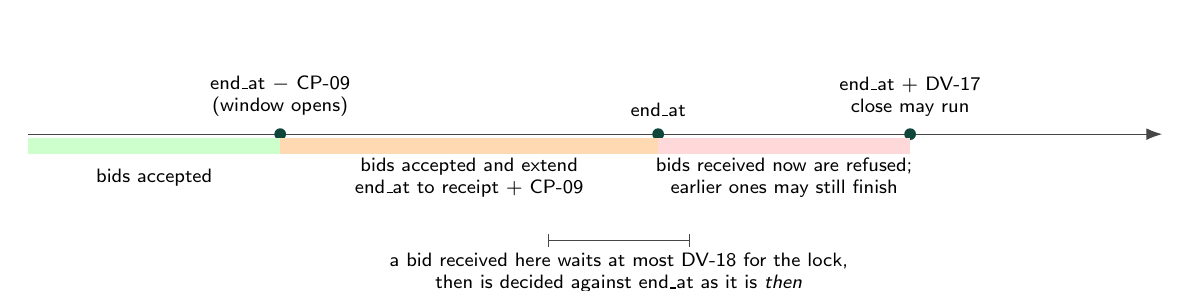
\begin{tikzpicture}[font=\sffamily\scriptsize,
  ev/.style={circle, fill=headcolor, inner sep=1.5pt},
  lb/.style={align=center, font=\sffamily\scriptsize}]
\draw[-{Latex[length=2mm]}, draw=edge] (0,0) -- (14.4,0);
\node[ev] (w) at (3.2,0) {}; \node[lb, above=3pt] at (w) {end\_at $-$ CP-09\\(window opens)};
\node[ev] (e) at (8.0,0) {}; \node[lb, above=3pt] at (e) {end\_at};
\node[ev] (g) at (11.2,0) {}; \node[lb, above=3pt] at (g) {end\_at $+$ DV-17\\close may run};
\fill[green!20] (0,-0.25) rectangle (3.2,-0.05); \fill[orange!30] (3.2,-0.25) rectangle (8.0,-0.05); \fill[red!15] (8.0,-0.25) rectangle (11.2,-0.05);
\node[lb] at (1.6,-0.55) {bids accepted};
\node[lb] at (5.6,-0.55) {bids accepted and extend\\end\_at to receipt $+$ CP-09};
\node[lb] at (9.6,-0.55) {bids received now are refused;\\earlier ones may still finish};
\draw[|-|, draw=edge] (6.6,-1.35) -- node[below=1pt, lb]{a bid received here waits at most DV-18 for the lock,\\then is decided against end\_at as it is \emph{then}} (8.4,-1.35);
\end{tikzpicture}
\caption{The end of an auction. Acceptance depends only on the receipt time; the close waits long enough for every bid received before the end to be decided.}
\label{fig:timing}
\end{figure}

\begin{itemize}[nosep]
  \item \textbf{Receipt time.} The BidService opens the database transaction as soon as the request has passed its checks, and \texttt{place\_bid} takes \texttt{now()}, the transaction's start time, as the receipt time. All instances therefore use one clock, the database server's (AS-2), and the time is fixed before any waiting for the lock. A bid is accepted only if its receipt time is before \texttt{end\_at} as it stands when the bid is decided (FR-AUC-04). Because extensions only ever move \texttt{end\_at} later, a bid received before the end is never refused because it waited.
  \item \textbf{Anti-sniping.} A bid received within CP-09 of \texttt{end\_at} sets \texttt{end\_at} to receipt $+$ CP-09 (FR-AUC-05). Every accepted bid in the window extends, including one immediately outbid by a proxy, because it is a valid bid.
  \item \textbf{Bounded wait and close grace.} Each bid waits at most DV-18 (1 second) for the auction row lock. The closer acts only after \texttt{end\_at} $+$ DV-17 (2 seconds), which is longer than DV-18. So when the close decides, every bid received before the end has already been decided or has timed out with a ``try again'' answer. A late extension pushes \texttt{end\_at} on, and the closer, which re-reads it under the lock, simply waits for the new time.
  \item \textbf{Processing order.} Bids are decided one at a time in the order they obtain the lock; the bid id, assigned under the lock, records that order. Receipt order can differ, because a bid received earlier may wait longer. The concurrency tests saw between 3 and 10 such cases per run of 300 bids. Replays (for history and after a void) therefore follow bid-id order. An earlier draft replayed in receipt order, and under contention its replay disagreed with the live decisions on 11 of 31 bids. That draft was corrected, and the tests now check that replay equals the live decisions in every run.
\end{itemize}

\subsection{Placing a bid}
\label{sec:placing}
\begin{enumerate}[nosep]
  \item \textbf{BidService}, before the lock:
  \begin{itemize}[nosep]
    \item authenticates the bidder and calls \texttt{IdentityQuery.assertCanTransact(bid)}: verified, e-mail verified, not suspended;
    \item consumes the bid rate limit CP-35 (FR-AUC-17);
    \item checks the listing is visible.
  \end{itemize}
  The proxy's automatic answers are part of a bid's own decision, so they consume no rate limit.
  \item \textbf{One transaction} calls \texttt{auctions.place\_bid(auction, bidder, maximum)}. Under the row lock, the function:
  \begin{itemize}[nosep]
    \item checks the status, start and end times, that the bidder is not the seller, and any restriction;
    \item applies \texttt{resolve} and anti-sniping;
    \item assigns the bidder's alias, records the bid and updates the auction, incrementing \texttt{version};
    \item locks the listing on the first bid (FR-LST-07).
  \end{itemize}
  \item \textbf{After commit}, the LiveBroadcaster:
  \begin{itemize}[nosep]
    \item emits \texttt{auction.state} to the room;
    \item sends \texttt{auction.outbid} to the previous leader if the lead changed;
    \item writes \texttt{auctions.bid.outbid} for the notification history.
  \end{itemize}
  The response to the bidder goes out at the same time.
\end{enumerate}
The broadcast is a best-effort message published after commit. A missed message is harmless, because the next message carries a higher sequence number and full state, and reconnecting clients re-fetch the state. Only the outbid event, which feeds the notification history, goes through the outbox.

\subsection{Voids and recomputation}
\label{sec:void}
An operator voids a bid only with a reason, on evidence of fraud or account compromise (FR-AUC-10). \texttt{auctions.recompute} then replays the remaining bids in processing order through \texttt{resolve} and sets the auction to the result, as if the voided bids had never been placed. Bidders whose position changed are notified.

The end time is \emph{not} shortened: an extension caused by a voided bid stays, because other bidders may already have acted on it. A remaining bid that would no longer be valid on replay, which is possible only after a void, is kept in the record but shown as not counted.

\subsection{Closing and second chance}
\label{sec:close}
\label{sec:second}
The AuctionCloser runs every few seconds over auctions due by \texttt{end\_at} $+$ DV-17, with \texttt{SKIP LOCKED}. For each, one transaction:
\begin{enumerate}[nosep]
  \item calls \texttt{auctions.close\_if\_due}, which re-checks the state under the lock and returns \texttt{awarded}, \texttt{unsold} or the existing status, so a repeated run has no effect;
  \item if awarded, calls \texttt{OrdersPort.createAuctionOrder} in the same transaction (DC-13), so an award without an order, or an order without an award, cannot exist;
  \item if unsold, moves the listing to \texttt{ended\_unsold};
  \item writes the events and audits.
\end{enumerate}

When Unit~2 reports \texttt{orders.order.payment\_expired} for a winner:
\begin{itemize}[nosep]
  \item \texttt{auctions.record\_strike} records the strike, at most once per order, and applies the bidding restriction once CP-12 is reached (FR-AUC-16).
  \item \texttt{auctions.next\_second\_chance} chooses the next eligible bidder. That is the highest maximum among bidders who have not won or been offered the item, whose bids are not voided and who are not restricted, with ties going to the earlier bidder. The offer is at that bidder's highest bid and expires after CP-11.
  \item If the offer is accepted, a \texttt{second\_chance} order is created. If it is declined or expires, the next bidder is tried. When none remain, the listing ends \texttt{ended\_unsold} and the seller may relist (FR-AUC-15).
  \item Identity eligibility (verified and not suspended) is checked again on acceptance.
\end{itemize}

\subsection{Shill-bidding flags}
\label{sec:shill}
The ShillDetector (Should, FR-AUC-18) runs after each auction closes and every few minutes on open auctions with many bids. It never blocks a bid; it raises flags with a score for the operator queue. It looks for:
\begin{itemize}[nosep]
  \item several bidders verified within the last 7 days placing small increments;
  \item bidders linked to the seller by device, payout account or payment instrument (from the Unit~1 and Unit~2 ports, FR-TNS-08);
  \item a bidder who repeatedly bids only in the last seconds across auctions;
  \item a bidder who raises the price against the same seller's other bidders but never wins.
\end{itemize}
While a flag on an auction is open, an operator may see its bidders' maximums; every such view is audited (FR-AUC-08).
\section{Listings}

\subsection{Life cycle}
\label{sec:lifecycle}
\begin{figure}[!htbp]
\centering
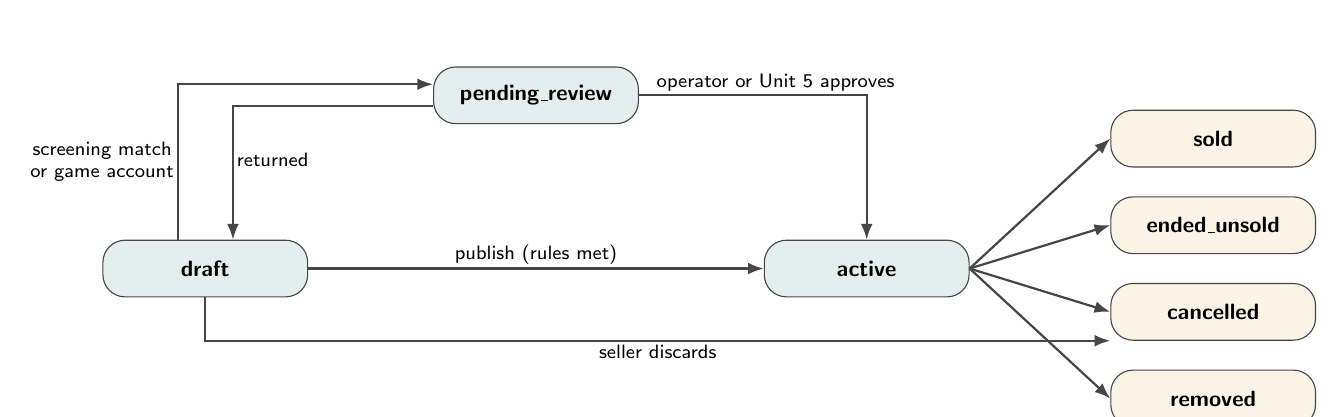
\begin{tikzpicture}[font=\sffamily\footnotesize,
  st/.style={draw=edge, rounded corners=8pt, fill=boxa, minimum width=2.6cm, minimum height=0.72cm, font=\sffamily\footnotesize\bfseries},
  tst/.style={st, fill=boxc},
  tr/.style={-{Latex[length=2mm]}, draw=edge, thick},
  lb/.style={font=\sffamily\scriptsize, align=center, fill=white, inner sep=1pt}]
\node[st] (d) at (0,0) {draft};
\node[st] (p) at (4.2,2.2) {pending\_review};
\node[st] (a) at (8.4,0) {active};
\node[tst] (s) at (12.8,1.65) {sold};
\node[tst] (u) at (12.8,0.55) {ended\_unsold};
\node[tst] (c) at (12.8,-0.55) {cancelled};
\node[tst] (r) at (12.8,-1.65) {removed};
\draw[tr] ([xshift=-10pt]d.north) |- node[lb, pos=0.25, left]{screening match\\or game account} ([yshift=4pt]p.west);
\draw[tr] ([yshift=-4pt]p.west) -| node[lb, pos=0.7, right]{returned} ([xshift=10pt]d.north);
\draw[tr] (p.east) -| node[lb, pos=0.3, above]{operator or Unit 5 approves} (a.north);
\draw[tr] (d) -- node[lb, above]{publish (rules met)} (a);
\draw[tr] (a.east) -- (s.west);
\draw[tr] (a.east) -- (u.west);
\draw[tr] (a.east) -- (c.west);
\draw[tr] (a.east) -- (r.west);
\draw[tr] (d.south) |- node[lb, pos=0.75, below]{seller discards} (c.south west);
\end{tikzpicture}
\caption{Listing status (FR-LST-12). Terminal states are shaded; relisting creates a new listing. An operator may also move a listing from \texttt{pending\_review} to \texttt{removed} (not drawn). The trigger \texttt{listing\_change} refuses every other change, and every change is written to \texttt{status\_history}.}
\label{fig:listing-states}
\end{figure}

\begin{itemize}[nosep]
  \item \textbf{Create.} Requires \texttt{@Verified(list)}. A draft records title, description, category, item kind and sale format. For physical items it also records condition, the defect declaration, the fulfilment options and, for courier, the parcel classes (FR-LST-01 to FR-LST-03). The location defaults to the seller's saved area, rounded to 3 decimal places of latitude and longitude (about 110~m); only the district name is shown (FR-LST-06).
  \item \textbf{Publish.} The ListingService:
  \begin{itemize}[nosep]
    \item takes an advisory lock on the seller, so two parallel publishes cannot both slip under the limit, then counts the seller's active listings against CP-28 (Pro status from Unit~2);
    \item runs the screening;
    \item moves the listing to \texttt{active}, or to \texttt{pending\_review} if a term matched or the item is a game account. Game accounts wait for Unit~5's ownership approval through \texttt{ListingsCommands}.
  \end{itemize}
  The database trigger then checks the photo and declaration rules. Publishing an auction also creates its auction row, with the start, reserve and duration (CP-07) and the increment and anti-sniping parameters copied from the current parameter version (FR-OPS-08).
  \item \textbf{Edit and clarify} (FR-LST-07). Until the first order or bid sets \texttt{locked\_at}, the seller may edit title, description and photos, and for fixed price also the price and quantity. After that the database refuses content changes, and the seller may only add clarifications, which are shown below the description with their time. An auction's start price, reserve and duration are never editable after publication.
  \item \textbf{Cancel} (FR-LST-08). A fixed-price listing can be cancelled while no unpaid or unfulfilled order holds a reservation, and an auction while it has no bids. An auction with bids can be cancelled only by an operator, with a reason, and every bidder is notified.
  \item \textbf{Visibility.} When Unit~1 reports a revoked verification or a suspension, all of the seller's listings get \texttt{seller\_visible = false}. They leave search, cannot be reserved and cannot be bid on; reinstatement restores them. Status is not changed, so nothing about the listing itself is lost (FR-SRC-04, FR-KYC-10, FR-TNS-05).
  \item \textbf{Relisting.} A seller who relists a similar item shortly after a cancelled or disputed sale is flagged for review (FR-TNS-02, Should). ``Similar'' means the same category with high title similarity (trigram), within 7 days.
\end{itemize}

\subsection{Photos}
\label{sec:media}
Listing photos are public, so unlike KYC images they are not encrypted, but they pass through the same checks as Unit~1's pipeline (SEC-INP-04, SEC-DAT-08):
\begin{enumerate}[nosep]
  \item the type is identified from the content (JPEG, PNG or WebP) and the size limit CP-33 applied;
  \item the image is decoded and rotated upright, and all metadata including EXIF location is removed;
  \item it is re-encoded at 1600 pixels on the long side, with a 400-pixel thumbnail (DV-20);
  \item it is stored under a random name on the \texttt{listing\_media} volume, served with a fixed content type and \texttt{nosniff}, and cached by the browser.
\end{enumerate}
Removing EXIF matters here: a phone photo of an item taken at home would otherwise publish the seller's home coordinates.

\subsection{AI-drafted text}
\label{sec:ai}
If the seller asks (FR-LST-13, Could), the photos are sent to the vision model behind \texttt{VisionDraftPort}, and the returned title and description are placed in the editor as a suggestion. Nothing is saved until the seller edits or accepts it and saves the draft. The listing records that a draft was used. The feature is switchable off and its failure never blocks listing creation.

% ------------------------------------------------------------------
\section{Search}
\label{sec:search}
\subsection{Text}
PostgreSQL has no Bangla stemmer, so the search vector uses the \texttt{simple} configuration. It splits text into words and lower-cases them without language-specific stemming, which works equally for Bangla and English (FR-SRC-01). Title words weigh more than description words. A \texttt{pg\_trgm} index on the title adds matching on parts of words and tolerates small misspellings, which matters for brand names written in either script.

The query combines the full-text match with a trigram match on the title, ranked by text rank and then recency. The tests confirm that a Bangla word (\textit{mobail} in Bangla script, ``mobile'') and an English word (\textit{samsung}) both find the same mixed-language listing.

\subsection{Filters, distance and sorting}
\begin{itemize}[nosep]
  \item \textbf{Filters} (FR-SRC-02): category, including sub-categories; item kind; sale format; price range, applied to the current price of auctions; condition; and maximum distance.
  \item \textbf{Distance.} A bounding box on the indexed rounded coordinates narrows the candidates, then the haversine distance \texttt{listings.distance\_km} is computed. The test confirms Dhaka to Chattogram at about 215~km. Distances are shown rounded to the kilometre, from rounded coordinates, so no exact location can be derived (FR-SRC-05). PostGIS was not chosen, because the precision needed is a kilometre and the extra extension is not worth the operational cost.
  \item \textbf{Sorting} (FR-SRC-03): newest, price ascending or descending, distance, and ending soonest (from \texttt{auctions\_due}).
  \item \textbf{Pagination} is by cursor, using the sort key and the id, so a page never repeats or skips a listing when new ones arrive.
  \item \textbf{What appears.} The view \texttt{listings.searchable} contains only active listings of visible sellers, and among auctions only open ones (FR-SRC-04). Guests use the same endpoint (FR-SRC-05).
\end{itemize}

\subsection{Featured listings and recommendations}
\label{sec:featured}
Up to DV-21 featured listings that match the query are shown above the results in a strip labelled ``Featured''. They are not mixed into the organic ranking, and each card is labelled wherever it appears (FR-MON-05). Recommendations (Could, FR-SRC-06) come from the user's recent categories and price band. They appear in their own labelled section, and never include featured placement unless it is labelled as such.

\subsection{Performance}
For the catalogue of 100{,}000 listings in NFR-PERF-05, the partial indexes cover only active listings of visible sellers:
\begin{itemize}[nosep]
  \item a GIN index on the search vector;
  \item a trigram index on the title;
  \item B-tree indexes on category and publication time, on price, and on the coordinates.
\end{itemize}
A load test with a generated catalogue of that size, and 1{,}000{,}000 stored bids for NFR-SCL-03, is part of the test plan.
\section{Performance and Scaling}
\begin{itemize}[nosep]
  \item \textbf{Bid latency} (NFR-PERF-02, 500~ms p95). The path is: authentication (one indexed session lookup, Unit~1), identity gate, rate-limit counter in Redis, and one database call that takes the lock. Inside the database the bid decision takes about 0.19~ms (measured over 500 bids). At the reference load of 20 bids per second on one auction, lock waits are therefore short; DV-18 caps them at 1~second.
  \item \textbf{Propagation} (NFR-PERF-03, 1~s p95). One message per committed change goes to the room through the Redis adapter, and each instance forwards it to its own sockets. The 200 viewers of the reference load are spread across instances.
  \item \textbf{Several instances} (NFR-SCL-01, NFR-SCL-02). No instance holds auction state: the database decides and Redis only carries messages. Any instance can serve any bid, and the closer runs safely on all instances at once (\texttt{SKIP LOCKED}).
  \item \textbf{Restart} (NFR-REL-01). The authoritative end time and the auction state are in PostgreSQL. Restarting the backend or Redis loses only connections, which reconnect and re-fetch the state.
  \item \textbf{Load test} (to run before the demonstration). A k6 script reproduces NFR-PERF-01: 500 signed-in users, 200 viewers and 20 bids per second on one auction for 60 seconds, 50 simultaneous purchases of a last unit, and search over 100{,}000 listings. It records p95 latencies and then runs the correctness checks of Appendix~\ref{app:tests} on the result (NFR-PERF-08).
\end{itemize}

\section{Security Design}
\begin{itemize}[nosep]
  \item \textbf{Authorisation.} Listing changes are allowed only for the seller and only in the states permitted. Bids require \texttt{@Verified(bid)}. Staff actions are limited to those listed in the API and each needs a reason and is audited (SEC-ACC-01 to SEC-ACC-03, FR-OPS-02).
  \item \textbf{Hidden data.} Maximums, the reserve amount, bidder identities and exact coordinates are never in an API response or a live message (SEC-WEB-05). The public history uses per-auction aliases. A bidder sees their own maximum through \texttt{/my-status}. Operators see maximums only while a fraud flag is open, and each view is audited (FR-AUC-08).
  \item \textbf{Abuse limits.} Bids are limited to 10 per minute per user per auction, listing creation to 10 per day, and search to 60 per minute per address (CP-35, SEC-ABU-01). The listing limit CP-28 is applied under an advisory lock.
  \item \textbf{Content.} Listing text is plain text, encoded on output (SEC-INP-03). Photos are re-encoded without metadata (Section~\ref{sec:media}). Prohibited categories cannot be chosen, and screening terms hold listings for review.
  \item \textbf{Integrity.} Bids are binding and cannot be edited or deleted. History tables are append-only. The application role cannot update them or delete bids (tested).
\end{itemize}

\section{Parameters}
\textbf{SRS parameters used:} CP-07 (durations); CP-08 (increment); CP-09 (anti-sniping); CP-10, CP-11 (payment and offer windows, applied by Unit~2 and here); CP-12 (strikes); CP-28 (listing limit); CP-33 (photos); CP-35 (rate limits); CP-37 (featured periods, display only).

\textbf{Design values introduced} (continuing DV-1 to DV-16):
\begin{dtable}{@{}>{\bfseries}p{1.3cm}>{\raggedright\arraybackslash}p{6.0cm}>{\raggedright\arraybackslash}p{2.6cm}>{\raggedright\arraybackslash}p{5.3cm}@{}}
\toprule
\textnormal{\textbf{ID}} & \textbf{Value} & \textbf{Default} & \textbf{Reason} \\ \midrule \endhead
DV-17 & Close grace after \texttt{end\_at} & 2 seconds & Must exceed DV-18 (Section~\ref{sec:timing}). \\
DV-18 & Maximum wait for an auction's lock & 1 second & Bounds latency; a timed-out bid is answered ``try again''. \\
DV-19 & Guest polling interval for auction state & 5 seconds & Guests have no live channel. \\
DV-20 & Listing photo sizes & 1600 px; thumbnail 400 px & Legible on phones; small downloads. \\
DV-21 & Featured listings shown above results & 3 & Visible, without crowding organic results. \\
DV-22 & Relisting similarity window & 7 days, title trigram similarity $\ge$ 0.6 & FR-TNS-02. \\
\bottomrule
\end{dtable}

\section{Testing}
\begin{dtable}{@{}>{\raggedright\arraybackslash}p{3.2cm}>{\raggedright\arraybackslash}p{12cm}@{}}
\toprule
\textbf{Level} & \textbf{Cases} \\ \midrule \endhead
Database (done) & 67 checks in \texttt{03\_listings\_auctions\_tests.sql}, each required to fail on its intended rule. They cover the listing rules; stock; increments; the worked bid example; ties; reserve lifting; anti-sniping; refusal after the end; strikes; bids being immutable; void and recompute; closing with grace; second chance; Bangla and English search; distance; visibility, including a hidden seller's auction refusing bids; and grants. The script is rerunnable. \\
Concurrency (done) & Four runs of 300 rising bids from 20 parallel connections. In each run lock order differed from receipt order for 3 to 10 bids, and every live decision equalled its replay. 50 buyers raced for 2 units: exactly 2 reservations (Appendix~\ref{app:tests}). \\
Unit & BidService gates (unverified, suspended, rate-limited); message sequence handling on the client; countdown offset; cursor pagination stability; screening matches in both scripts. \\
Integration & Close plus order creation is atomic (order failure rolls back the award). An outbid notice reaches only the previous leader. A reconnecting client re-fetches state. Listings are hidden on suspension and restored. Second-chance chain to exhaustion. \\
Load & The k6 script of the performance section, with the correctness checks afterwards (AC-1, AC-2). \\
\bottomrule
\end{dtable}

\section{Notes for Integration}
\begin{enumerate}[label=\textbf{I-\arabic*}, leftmargin=*, nosep]
  \setcounter{enumi}{13}
  \item \textbf{Unit 2.} \texttt{ListingsPort} is implemented by \texttt{listings.reserve}, \texttt{release} and \texttt{mark\_sold}. On an auction order being paid, the listing moves to \texttt{sold} through \texttt{markSold}. A refund after payment does not return stock automatically; the seller relists.
  \item \textbf{Unit 5} adds its game-account details table with a foreign key to \texttt{listings.listings} (allowed by DC-5), and approves listings through \texttt{ListingsCommands}.
  \item \textbf{Unit 6} delivers \texttt{auctions.bid.outbid} and the ending-soon notices (FR-NTF-02). Ending-soon notices are driven by \texttt{auctions\_due}.
  \item \textbf{Unit 7} hosts the queues for listings in review, flags and voids, using this unit's staff endpoints.
  \item \textbf{SRS clarifications proposed:}
  \begin{itemize}[nosep]
    \item the reserve-lifting rule of Section~\ref{sec:rules} (FR-AUC-09);
    \item guests see auction state by polling (IF-COM-02);
    \item an extension caused by a voided bid is kept (FR-AUC-10);
    \item add DV-17 to DV-22 to the SRS parameter table.
  \end{itemize}
\end{enumerate}

\appendix
\section{Traceability}
\label{app:trace}
{\small\begin{longtable}{@{}>{\ttfamily}p{2.4cm}>{\raggedright\arraybackslash}p{10.6cm}>{\raggedright\arraybackslash}p{2.2cm}@{}}
\toprule \textnormal{\textbf{Requirement}} & \textbf{Design element} & \textbf{Section} \\ \midrule \endhead
FR-LST-01 & Draft fields; kind and format fixed after publication (trigger) & \ref{sec:lifecycle}, \ref{sec:data} \\
FR-LST-02 & Two photos and defect photo or declaration (trigger) & \ref{sec:lifecycle}, \ref{sec:data} \\
FR-LST-03 & Parcel classes required for courier (constraint) & \ref{sec:data} \\
FR-LST-04 & Fixed price needs price and quantity & \ref{sec:data} \\
FR-LST-05 & Auction start, reserve $\ge$ start, duration CP-07, quantity 1 & \ref{sec:lifecycle}, \ref{sec:data} \\
FR-LST-06 & Rounded coordinates; district shown only & \ref{sec:lifecycle} \\
FR-LST-07 & \texttt{locked\_at}; content lock trigger; clarifications & \ref{sec:lifecycle} \\
FR-LST-08 & Cancellation rules; operator cancel with bids & \ref{sec:lifecycle}, \ref{sec:api} \\
FR-LST-09 & Listing limit under advisory lock; Pro status from Unit 2 & \ref{sec:lifecycle} \\
FR-LST-10 & Prohibited categories refused by trigger & \ref{sec:data} \\
FR-LST-11 & ScreeningService; \texttt{pending\_review} & \ref{sec:lifecycle} \\
FR-LST-12 & Status machine trigger; \texttt{status\_history} & \ref{sec:lifecycle} \\
FR-LST-13 & \texttt{VisionDraftPort}; never saved without the seller & \ref{sec:ai} \\
FR-SRC-01 & \texttt{simple} text search plus trigrams; Bangla and English tested & \ref{sec:search} \\
FR-SRC-02 & Filters; bounding box and haversine distance & \ref{sec:search} \\
FR-SRC-03 & Sorts; cursor pagination & \ref{sec:search} \\
FR-SRC-04 & \texttt{listings.searchable}; \texttt{seller\_visible} & \ref{sec:search}, \ref{sec:lifecycle} \\
FR-SRC-05 & Public search; rounded distances & \ref{sec:search} \\
FR-SRC-06 & Labelled recommendations & \ref{sec:featured} \\
FR-AUC-01 & \texttt{end\_at} in PostgreSQL; client offset from \texttt{serverTime} & \ref{sec:live}, \ref{sec:timing} \\
FR-AUC-02 & BidService gates; \texttt{place\_bid} checks; minimum & \ref{sec:placing}, \ref{sec:rules} \\
FR-AUC-03 & Row lock in \texttt{place\_bid}; processing order & \ref{sec:why-db}, \ref{sec:timing} \\
FR-AUC-04 & Receipt time \texttt{now()}; refusal at or after \texttt{end\_at} & \ref{sec:timing} \\
FR-AUC-05 & Extension to receipt $+$ CP-09 & \ref{sec:timing} \\
FR-AUC-06 & \texttt{auctions.resolve} proxy rules & \ref{sec:rules} \\
FR-AUC-07 & Ties to the earlier maximum; price rule checked & \ref{sec:rules} \\
FR-AUC-08 & Maximums never returned; flag-gated, audited staff view & \ref{sec:shill}, \ref{sec:api} \\
FR-AUC-09 & Reserve lifting; unsold when not met & \ref{sec:rules}, \ref{sec:close} \\
FR-AUC-10 & Immutable bids; void and replay in processing order & \ref{sec:void} \\
FR-AUC-11 & \texttt{auction.state} with sequence numbers & \ref{sec:live} \\
FR-AUC-12 & \texttt{auction.outbid} to the previous leader & \ref{sec:live}, \ref{sec:placing} \\
FR-AUC-13 & Aliases; history from replay & \ref{sec:rules}, \ref{sec:data} \\
FR-AUC-14 & Close plus \texttt{createAuctionOrder} in one transaction & \ref{sec:close} \\
FR-AUC-15 & \texttt{next\_second\_chance}; offers; exhaustion to unsold & \ref{sec:close} \\
FR-AUC-16 & \texttt{record\_strike}; restrictions checked in \texttt{place\_bid} & \ref{sec:close} \\
FR-AUC-17 & Bid rate limit before the lock; proxy answers not limited & \ref{sec:placing} \\
FR-AUC-18 & ShillDetector flags; no automatic blocking & \ref{sec:shill} \\
FR-FIX-02 & \texttt{listings.reserve}: one conditional update & \ref{sec:data}, \ref{app:tests} \\
FR-FIX-04 & \texttt{mark\_sold}; ``currently reserved'' in the view & \ref{sec:data} \\
FR-FIX-05 & Definite answer per request; race test 2 of 50 & \ref{app:tests} \\
FR-MON-05 & Featured strip, always labelled & \ref{sec:featured} \\
FR-KYC-10 & Listings hidden on revocation & \ref{sec:lifecycle} \\
FR-TNS-05 & Listings hidden on suspension & \ref{sec:lifecycle} \\
FR-TNS-02 & Relisting similarity flag & \ref{sec:lifecycle} \\
FR-TNS-08 & Linked-account signal in shill scoring & \ref{sec:shill} \\
SEC-ABU-01 & Bid, listing and search limits & \ref{sec:api}, \ref{sec:placing} \\
SEC-WEB-05 & Hidden fields never returned & \ref{sec:api} \\
SEC-DAT-08 & EXIF removed from listing photos & \ref{sec:media} \\
SEC-INP-04 & Photo checks and re-encoding & \ref{sec:media} \\
SEC-SES-07 & Live channel on Unit 1's authenticated socket & \ref{sec:live} \\
IF-UI-03 & Listing, search and auction endpoints and live state & \ref{sec:api}, \ref{sec:live} \\
IF-COM-02 & Re-fetch on reconnect; guests poll & \ref{sec:live} \\
NFR-PERF-01 & Load-test plan at the reference load & \ref{sec:api} \\
NFR-PERF-02 & One database call per bid (0.19 ms measured) & \ref{sec:why-db} \\
NFR-PERF-03 & One message per change through the Redis adapter & \ref{sec:live} \\
NFR-PERF-05 & Partial GIN, trigram and B-tree indexes & \ref{sec:search} \\
NFR-PERF-08 & Correctness checks after concurrency tests & \ref{app:tests} \\
NFR-REL-01 & State in PostgreSQL; Redis only carries messages & \ref{sec:why-db} \\
NFR-REL-03 & Closer idempotent with SKIP LOCKED & \ref{sec:close} \\
NFR-SCL-01 & Socket.IO Redis adapter & \ref{sec:live} \\
NFR-SCL-02 & No instance-local state & \ref{sec:why-db} \\
NFR-SCL-03 & Load test with 100{,}000 listings and 1{,}000{,}000 bids & \ref{sec:search} \\
NFR-USE-01 & Rules link on the auction page; refusal codes explain & \ref{sec:api} \\
DR-03 & \texttt{snapshot} for orders & \ref{sec:api} \\
DR-04 & \texttt{auctions.bids} with maximums and receipt time & \ref{sec:data} \\
DR-10 & Append-only histories; immutable bids & \ref{sec:data} \\
\bottomrule\end{longtable}}


\section{Database Schema and Tests}
\label{app:ddl}
\subsection{Test results}
\label{app:tests}
Loaded after the Unit~1 and Unit~2 schemas in PostgreSQL 16, using PostgreSQL 15 features only. Every check passed. The concurrency results follow the script output.
{\scriptsize
\begin{verbatim}
PASS  FR-LST-10 a prohibited category cannot be used [is prohibited]
PASS  category must match the item kind [does not match item kind]
PASS  a new listing starts as a draft [starts as draft]
PASS  FR-LST-05 an auction has quantity 1 [auction_single_unit]
PASS  FR-LST-03 courier needs weight and size classes [courier_needs_parcel]
PASS  a game account has no physical fields [game_fields]
PASS  FR-LST-02 publishing needs at least two photos [at least two photos]
PASS  FR-LST-02 a defect photo or a no-defects declaration is required [declare that there are none]
PASS  a listing with two photos, one showing defects, is published
PASS  FR-LST-01 sale format is fixed after publication [fixed after publication]
PASS  reserve 2 of 3
PASS  reserving 2 more of the 1 left is refused
PASS  reserve the last unit
PASS  searchable view shows the listing as currently reserved
PASS  after a release and a sale: 1 available, 0 reserved, 2 sold, still active
PASS  FR-FIX-04 sold when nothing is available or reserved
PASS  stock must always add up [stock_adds_up]
PASS  FR-LST-07 content is locked after the first order [locked after the first bid or order]
PASS  FR-LST-12 sold is terminal [is not permitted]
PASS  clarifications are append-only [append-only]
PASS  increment on BDT 10,000 is 2% = BDT 200
PASS  increment on BDT 1,000 is the BDT 50 minimum
PASS  2% is rounded up to a whole taka (BDT 12,345.67 -> BDT 247)
PASS  first bid leads at the starting price, whatever the maximum
PASS  FR-AUC-02 a bid below price + increment is refused [below_minimum]
PASS  FR-AUC-06 the leader's proxy answers a lower maximum: price = 1,200 + 50
PASS  FR-AUC-07 equal maximums: the earlier one wins, at that maximum
PASS  leader is still the first bidder after the tie
PASS  a higher maximum takes the lead at the old maximum + increment (1,500 + 50)
PASS  a leader can only raise their maximum [max_not_higher]
PASS  raising one's own maximum does not raise the price
PASS  FR-AUC-02 the seller cannot bid [seller_cannot_bid]
PASS  FR-AUC-13 consistent masks: bidders are 1, 2, 3 in order of first bid
PASS  FR-AUC-08 the public history never shows the leader's maximum (250,000 or 200,000)
PASS  recorded live decisions equal a replay of the same bids
PASS  a maximum above the reserve lifts the price to the reserve
PASS  "reserve not met" is cleared
PASS  below the reserve: price stays at the start and "reserve not met" shows
PASS  a bid in the last 2 minutes extends the end to receipt + 2 minutes
PASS  the end time only ever moves later
PASS  FR-AUC-04 a bid received at or after the end is refused [auction_ended]
PASS  one strike does not restrict
PASS  the second strike in 90 days restricts bidding for 30 days
PASS  a restricted bidder is refused [bidder_restricted]
PASS  a bid cannot be changed [can only be voided]
PASS  a bid cannot be deleted [cannot be deleted]
PASS  a bid can be voided only once [only be voided, once]
PASS  FR-AUC-10 after the void the auction is as if those bids never happened
PASS  not closed before end + grace
PASS  the due auction closes as awarded
PASS  awarded to the leader at the current price
PASS  FR-AUC-09 reserve not met closes unsold
PASS  closing again changes nothing
PASS  an award below the reserve is impossible [award_meets_reserve]
PASS  the next eligible bidder is Babu at BDT 1,500
PASS  no further eligible bidder after Babu has been offered
PASS  only one open offer per auction [offer_one_open]
PASS  FR-SRC-01 a Bangla word finds the listing
PASS  FR-SRC-01 an English word finds the same listing
PASS  a part of a word matches through trigrams (galax)
PASS  FR-SRC-02 Dhaka to Chattogram is about 215 km (rounded coordinates)
PASS  closed auctions and sold listings are not searchable
PASS  FR-SRC-04 listings of a suspended or unverified seller disappear from search
PASS  FR-TNS-05 a hidden seller's auction takes no bids [listing not available]
PASS  FR-FIX-05 and FR-SRC-04 a hidden seller's stock cannot be reserved
PASS  application role cannot rewrite listing history [permission denied]
PASS  application role cannot delete bids [permission denied]

Concurrency tests on the final schema (separate connections, one transaction per bid):
  A. Four runs, each 20 bidders x 15 rising bids on one auction in parallel, with random
     delays so that lock order differs from receipt order:
       accepted 32 / 36 / 34 / 35; processed out of receipt order 3 / 10 / 8 / 9;
       in every run: every recorded decision equals the replay; the price never decreased;
       the leader holds the highest maximum; final price = min(top maximum,
       second maximum + increment).
  B. 50 buyers reserving the last 2 units at once: 2 granted, 48 refused.
  Found and fixed while testing: an earlier replay ordered bids by receipt time; under
  contention it disagreed with the live decisions on 11 of 31 bids.
  Timing: place_bid takes about 0.19 ms per call inside the database (500 accepted bids,
  one session, excluding network and commit).
\end{verbatim}
}

\subsection{Schema}
\lstinputlisting[language=SQLpg]{sql/03_listings_auctions.sql}
\end{document}
